\documentclass[14pt]{extarticle}
\usepackage{fontspec}
\usepackage{polyglossia}
\usepackage{amsmath}
\usepackage{amssymb}
\usepackage{xcolor}
\usepackage{fancyhdr}
\usepackage{graphicx}
\usepackage{listings}
\usepackage[most]{tcolorbox}
% \usepackage{setspace}
\usepackage{pifont}
\usepackage{enumitem}
\usepackage{titlesec}
\usepackage[bottom]{footmisc}
\usepackage{titling}
\usepackage{minted}
\usepackage{etoolbox}
\usepackage{array}
\usepackage{extsizes}
\usepackage{float}
\usepackage{booktabs}
\usepackage{hyperref}
\usepackage[onehalfspacing]{setspace}
\usepackage[a4paper, top=2.7cm, bottom=2.7cm, left=2.5cm, right=2.5cm, headheight=1.5cm, headsep=0.5cm]{geometry}
\usepackage{tikz}

\usetikzlibrary{automata, positioning, arrows.meta, arrows}

\newfontfamily\emoji{Segoe UI Emoji}

\pagestyle{fancy}

\setmainlanguage[numerals=western]{arabic}
\setotherlanguage{english}
% \newfontfamily\arabicfont[Script=Arabic]{Amiri}
\newfontfamily\arabicfont[Script=Arabic]{Calibri}
\newfontfamily\arabicfonttt[Script=Arabic]{Courier New}

\lstset{
  language=[Sharp]C,
  numbers=left,
  stepnumber=1,
  numbersep=8pt,
  frame=single,
  basicstyle=\ttfamily\small,
  keywordstyle=\color{blue},
  stringstyle=\color{red},
  commentstyle=\color{green!50!black}
}

\newif\ifdetailed
\ifdefined\setdetailed
  \setdetailed
\fi

\newif\ifwithsols
\ifdefined\setwithsols
  \setwithsols
\fi

% unified tcolorboxes for articles
\tcbset{colback=white, colframe=black, fonttitle=\bfseries, boxrule=0.8pt}
\newtcolorbox{boxDef}[1][]{colback=blue!5!white,colframe=blue!75!black,
  title={{\emoji📘} تعريف\ifx\\#1\\\else ~#1\fi :}}
\newtcolorbox{boxExercise}[1][]{colback=cyan!5!white,colframe=cyan!70!black,
  title={{\emoji🧩} تمرين\ifx\\#1\\\else ~#1\fi :}}
\newtcolorbox{boxExample}[1][]{colback=yellow!5!white,colframe=orange!90!black,
  title={{\emoji📝} مثال\ifx\\#1\\\else ~#1\fi :}}
\newtcolorbox{boxNote}[1][]{colback=gray!10!white,colframe=black,
  title={{\emoji✨} ملاحظة\ifx\\#1\\\else ~#1\fi :}}
\newtcolorbox{boxAttention}[1][]{colback=magenta!10!white,colframe=magenta!80!black,
  title={{\emoji🔔} تنبيه\ifx\\#1\\\else ~#1\fi :}}
\newtcolorbox{boxWarning}[1][]{colback=red!5!white,colframe=red!75!black,
  title={{\emoji⚡} ملاحظة هامة\ifx\\#1\\\else ~#1\fi :}}
\newtcolorbox{boxSolution}[1][]{colback=green!5!white,colframe=green!60!black,
  title={{\emoji✅} حل\ifx\\#1\\\else ~#1\fi :}}
\newtcolorbox{boxSymbol}[1][]{colback=purple!5!white,colframe=purple!70!black,
  title={{\emoji🔣} رمز\ifx\\#1\\\else ~#1\fi :}}
\newtcolorbox{boxHint}[1][]{colback=teal!5!white,colframe=teal!60!black,
  title={{\emoji💡} تلميح\ifx\\#1\\\else ~#1\fi :}}


\tcbset{simplecode/.style={ colback=gray!5, colframe=black!50, boxrule=0.4pt, arc=2pt, left=4pt,right=4pt,top=4pt,bottom=4pt}}
\newenvironment{boxCode}{\begin{tcolorbox}[simplecode]}{\end{tcolorbox}}

\newcolumntype{C}[1]{>{\centering\arraybackslash}p{#1}}

% redefine spaces after titles
\makeatletter
\renewcommand{\@maketitle}{%
  \begin{center}
    {\huge \bfseries \@title \par}%
    \vskip 0.2em % space between title and author
    {\large \@author \par}%
    % \vskip 0.2em % space between author and date
    % {\normalsize \@date \par}%
  \end{center}
}
\makeatother

\fancyhf{} % clear default
\fancypagestyle{plain}{
  \fancyhf{}
  \fancyhead[L]{مدرسة التسامح الشاملة}
  % \fancyhead[L]{
\includegraphics[height=1cm]{../../../images/logoTasamoh.png}}
  \fancyhead[R]{الأستاذ محمود اغبارية}
  \fancyfoot[C]{\thepage}
}

\fancyhead[L]{مدرسة التسامح الشاملة}
\fancyhead[R]{الأستاذ محمود اغبارية}
\fancyfoot[C]{\thepage}
% \date{\today}

\setcounter{tocdepth}{3} % only section subsection and subsubsection in TOC

\newcommand{\importpdfpage}[2]{%
    \thispagestyle{empty}
    \newgeometry{left=0cm,right=0cm,top=0cm,bottom=0cm}
    \includegraphics[page=#2,width=0.95\paperwidth,height=0.95\paperheight,keepaspectratio]{#1}
    \restoregeometry
}

\newcommand{\insertFullImg}[1]{%
    \noindent
    \makebox[\textwidth][c]{
        \includegraphics[width=0.9\paperwidth,keepaspectratio]{#1}%
    }%
}%

% ----------------------


% \begin{document}

% \maketitle

% % \clearpage  % start TOC on a new page
% % \renewcommand{\contentsname}{جدول المحتويات}
% % \tableofcontents
% % \clearpage

% \part*{part 1} % the * prevents numbering
% \section*{مقدمة}
% \subsection*{مثال رياضي}
% \subsubsection*{مثال فرعي}
% \paragraph*{ paragraph 1}
% \subparagraph*{sub paragraph 1}

% \ifdetailed
% \begin{english}
% \begin{minted}{csharp}
% // C# Example
% \end{minted}
% \end{english}
% \fi

% OLD WAY
% \ifdetailed
% \begin{english}
% \begin{lstlisting}
% // C# Example
% \end{lstlisting}
% \end{english}
% \fi

% % 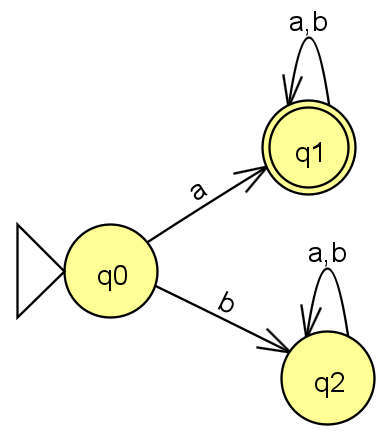
\includegraphics[width=0.2\textwidth]{../../../images/DFAs/ex1_q1.png}



% \vspace{3cm}
% \begin{flushleft}
% أرجو لكم وقتًا ممتعًا.

% الأستاذ محمود اغبارية.
% \end{flushleft}


% \end{document}


\ifwithsols
\title{حل ورقة تمرن 1 ب للصف العاشر 10 - أخطاء وتتبع الكود}
\else
\title{ورقة تمرن 1 ب للصف العاشر 10 - أخطاء وتتبع الكود}
\fi

\begin{document}

\maketitle
\thispagestyle{fancy}

\section*{القسم الأوّل: اكتشاف الأخطاء}
اشرح ما هو الخطأ في كلّ من المقاطع البرمجية التالية:

\begin{enumerate}[itemsep=2em]

% 1. Declare twice
\begin{english}
\item
\begin{minted}{csharp}
int num = 5;
int num = 10;
Console.WriteLine(num);
\end{minted}
\end{english}
\ifwithsols
\begin{boxSolution}
الخطأ: تم تعريف المتغيّر \textenglish{num} مرتين باستخدام كلمة \textenglish{int}. لا يمكن تعريف نفس المتغيّر أكثر من مرّة في نفس المجال. \\
التصحيح: لإعطاء قيمة جديدة للمتغيّر الموجود، نكتب \textenglish{num = 10;} بدون كلمة \textenglish{int}.
\end{boxSolution}
\fi

% 2. Mismatched type
\begin{english}
    \item
\begin{minted}{csharp}
int age = 15.5;
Console.WriteLine(age);
\end{minted}
\end{english}
\ifwithsols
\begin{boxSolution}
الخطأ: تم إعطاء قيمة عشرية \textenglish{(15.5)} لمتغيّر من نوع عدد صحيح \textenglish{(int)}. \\
التصحيح: إما تغيير القيمة إلى عدد صحيح (مثلاً 15)، أو تغيير نوع المتغيّر إلى \textenglish{double}.
\end{boxSolution}
\fi

% 3. Use without declaration
\begin{english}
    \item
\begin{minted}{csharp}
sum = 10 + 20;
Console.WriteLine(sum);
\end{minted}
\end{english}
\ifwithsols
\begin{boxSolution}
الخطأ: تم استخدام المتغيّر \textenglish{sum} وإعطائه قيمة دون تعريفه أولاً (أي دون تحديد نوعه). \\
التصحيح: يجب كتابة \textenglish{int sum = 10 + 20;} في السطر الأول.
\end{boxSolution}
\fi

% 4. Illegal name (number)
\begin{english}
    \item
\begin{minted}{csharp}
int 1number = 5;
Console.WriteLine(1number);
\end{minted}
\end{english}
\ifwithsols
\begin{boxSolution}
الخطأ: اسم المتغيّر \textenglish{1number} يبدأ برقم، وهذا ممنوع في لغة \textenglish{C\#}. \\
التصحيح: كتابة الاسم بحيث يبدأ بحرف، مثل \textenglish{number1}.
\end{boxSolution}
\fi

% 5. Illegal name (space)
\begin{english}
    \item
\begin{minted}{csharp}
int my age = 15;
Console.WriteLine(my age);
\end{minted}
\end{english}
\ifwithsols
\begin{boxSolution}
الخطأ: اسم المتغيّر \textenglish{my age} يحتوي على مسافة (فراغ)، وهذا غير مسموح في تسمية المتغيّرات. \\
التصحيح: استخدام اسم متصل، مثل \textenglish{myAge} أو \textenglish{my\_age}.
\end{boxSolution}
\fi

\end{enumerate}

\clearpage

\section*{القسم الثاني: تتبع الكود}
ما هو ناتج (مخرجات) المقاطع البرمجية التالية على الشاشة؟

\begin{enumerate}[resume, itemsep=2em]

\item
بافتراض أن المستخدم أدخل الرقم $5$، ثم الرقم $10$:
\begin{english}
\begin{minted}{csharp}
int a = int.Parse(Console.ReadLine());
int b = int.Parse(Console.ReadLine());
Console.WriteLine(a);
Console.WriteLine(b);
\end{minted}
\end{english}
\ifwithsols
\begin{boxSolution}
\begin{english}
\begin{minted}{text}
5
10
\end{minted}
\end{english}
\end{boxSolution}
\fi

\item
بافتراض أن المستخدم أدخل الرقم $2.5$، ثم الرقم $3.5$:
\begin{english}
\begin{minted}{csharp}
double x = double.Parse(Console.ReadLine());
double y = double.Parse(Console.ReadLine());
Console.WriteLine(x + y);
\end{minted}
\end{english}
\ifwithsols
\begin{boxSolution}
\begin{english}
\begin{minted}{text}
6
\end{minted}
\end{english}
\end{boxSolution}
\fi

\item
بافتراض أن المستخدم أدخل الأرقام التالية بالتوالي: $4$ ثم $1.5$:
\begin{english}
\begin{minted}{csharp}
int num1 = int.Parse(Console.ReadLine());
double num2 = double.Parse(Console.ReadLine());
Console.WriteLine(num1 + 1);
Console.WriteLine(num2 * 2);
\end{minted}
\end{english}
\ifwithsols
\begin{boxSolution}
\begin{english}
\begin{minted}{text}
5
3
\end{minted}
\end{english}
\end{boxSolution}
\fi

\item
بافتراض أن المستخدم أدخل الأرقام التالية بالتوالي: $7$ ثم $9$:
\begin{english}
\begin{minted}{csharp}
int x = int.Parse(Console.ReadLine());
Console.WriteLine(x);
x = int.Parse(Console.ReadLine());
Console.WriteLine(x);
\end{minted}
\end{english}
\ifwithsols
\begin{boxSolution}
\begin{english}
\begin{minted}{text}
7
9
\end{minted}
\end{english}
\end{boxSolution}
\fi

\item
بافتراض أن المستخدم أدخل الأرقام: $3$، $4$، $5$ بالتوالي:
\begin{english}
\begin{minted}{csharp}
int a = int.Parse(Console.ReadLine());
int b = int.Parse(Console.ReadLine());
int c = int.Parse(Console.ReadLine());
int sum = a + b + c;
Console.WriteLine(sum);
Console.WriteLine(sum / 3.0);
\end{minted}
\end{english}
\ifwithsols
\begin{boxSolution}
\begin{english}
\begin{minted}{text}
12
4
\end{minted}
\end{english}
\end{boxSolution}
\fi

\end{enumerate}

\clearpage

\section*{القسم الثالث: أسئلة مفاهيمية أساسية}

\begin{enumerate}[resume, itemsep=2em]

\item
حدّد ما إذا كانت الجمل التالية صحيحة أم خاطئة:
\begin{enumerate}
    \item يمكن تغيير قيمة المتغيّر بعد تعريفه في لغة \textenglish{C\#}.
    \item يمكن تغيير نوع المتغيّر (مثلاً من \textenglish{int} إلى \textenglish{string}) بعد تعريفه.
    \item يمكن تعريف متغيرين مختلفين بنفس الاسم في نفس البرنامج.
\end{enumerate}
\ifwithsols
\begin{boxSolution}
\begin{enumerate}
    \item صحيحة (تسمى متغيّرات لأن قيمتها يمكن أن تتغيّر).
    \item خاطئة (نوع المتغيّر ثابت بمجرد تعريفه ولا يمكن تغييره).
    \item خاطئة (يجب أن يكون لكل متغيّر اسم فريد خاص به في نفس النطاق).
\end{enumerate}
\end{boxSolution}
\fi

\item
ما هو نوع المتغيّر المناسب لحفظ كلّ من البيانات التالية؟ (\textenglish{int} أم \textenglish{double})
\begin{enumerate}
    \item عدد الطلاب في الصف.
    \item وزن الإنسان بالكيلوغرام.
    \item علامة الطالب في الامتحان (مثلاً 95.5).
    \item عدد أيام الأسبوع.
\end{enumerate}
\ifwithsols
\begin{boxSolution}
\begin{enumerate}
    \item \textenglish{int}
    \item \textenglish{double}
    \item \textenglish{double}
    \item \textenglish{int}
\end{enumerate}
\end{boxSolution}
\fi

\item
اكتب أمرًا برمجيًا لتعريف متغيّر باسم \textenglish{score} من نوع عدد صحيح، وأعطه القيمة البدائية $100$.
\ifwithsols
\begin{boxSolution}
\begin{english}
\begin{minted}{csharp}
int score = 100;
\end{minted}
\end{english}
\end{boxSolution}
\fi

\item
اكتب أمرًا برمجيًا لتعريف متغيّر باسم \textenglish{price} من نوع عدد عشري، وأعطه القيمة البدائية $45.99$.
\ifwithsols
\begin{boxSolution}
\begin{english}
\begin{minted}{csharp}
double price = 45.99;
\end{minted}
\end{english}
\end{boxSolution}
\fi

\item
لديك المتغيّرات التالية:
\begin{english}
\begin{minted}{csharp}
int x = 5;
int y = 10;
\end{minted}
\end{english}
اكتب أوامر برمجية لتبديل القيم بين المتغيّرين \textenglish{x} و \textenglish{y} (بحيث تصبح قيمة \textenglish{x} تساوي $10$ وقيمة \textenglish{y} تساوي $5$).
\ifwithsols
\begin{boxSolution}
نحتاج إلى استخدام متغيّر وسيط (ثالث) لحفظ القيمة مؤقتًا:
\begin{english}
\begin{minted}{csharp}
int temp = x;
x = y;
y = temp;
\end{minted}
\end{english}
\end{boxSolution}
\fi

\end{enumerate}

\vspace{3cm}
\begin{flushleft}
أرجو لكم وقتًا ممتعًا.

الأستاذ محمود اغبارية.
\end{flushleft}

\end{document}
